In this chapter we move away from the ScatterNet ideas from the previous 
chapters and instead look at using the wavelet domain as a new space in which to
learn. In particular the ScatterNet, and even the learnable ScatterNet proposed
in the previous chapter, are built around taking complex magnitudes of the
highpass wavelets. This inherently builds invariance to shifts but at the cost
of making things smoother. In many ways this was beneficial, as it allowed us to
subsample the output and we saw that the scattering layers worked well right
before the downsampling stages of a CNN\@. However, we would now like to explore
if it is possible and at all beneficial to learn with wavelets without taking
the complex magnitude. This means that the frequency support of our activations
will remain in the same space in the Fourier domain.

The inspiration to this chapter is the hope that learning in the
frequency/wavelet domain may afford simpler filters than learning in the pixel
domain. A classic example of this is the first layer filters in AlexNet shown in
\autoref{fig:ch6:alexnet}. These are a collection of lowpass (with colour) and
oriented highpass filters, each of which would only require a few parameters if
coded as subband gains.

\begin{figure}[bt]
  \centering
  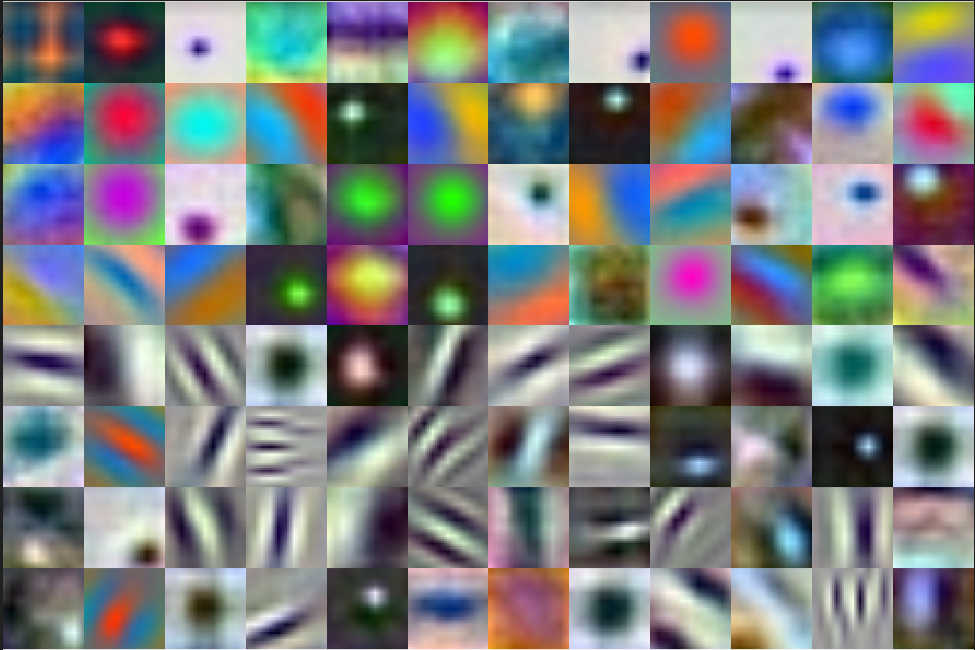
\includegraphics[width=0.7\textwidth]{\imgpath/alexfilters.png}
  \mycaption{First layer filters of the AlexNet architecture}{The first layer
  filters of the seminal AlexNet \cite{krizhevsky_imagenet_2012} are an
  inspiration for considering learning filters in the wavelet domain. Each of
  these $11\x 11$ filters would only require a handful of non zero coefficients
  in the wavelet domain. Weights taken from torchvision
  \cite{marcel_torchvision_2010}.}
  \label{fig:ch6:alexnet}
\end{figure}

Our experiments show that \ellipsis

As neural network training involves presenting thousands of training samples, we
want our layer to be fast. To achieve this we would ideally choose to use
a critically sampled filter bank implementation. The fast 2-D Discrete Wavelet
Transform (DWT) is a possible option, but it has two drawbacks: it has poor
directional selectivity and any alteration of wavelet coefficients will cause
the aliasing cancelling properties of the reconstructed signal to disappear.
Instead we choose to use the Dual-Tree Complex Wavelet Transform ($DTCWT$)
\cite{selesnick_dual-tree_2005} as at the expense of limited redundancy (4:1),
it enables us to have better directional selectivity, and allows us to modify
the wavelet coefficients and still have minimal aliasing terms when we
reconstruct \cite{kingsbury_complex_2001}.

% This work is a step
\autoref{sec:ch6:method} of the paper describes the implementation details of
our design, and \autoref{sec:ch6:results} describes the experiments and results
we have done so far.
